\section{Resultados y Análisis Experimental}
\label{sec:resultados}

En esta sección se presentan y discuten los resultados obtenidos en las mediciones de tiempo de CPU y memoria para los algoritmos de ordenamiento y multiplicación de matrices. Todos los gráficos expuestos corresponden a las figuras generadas automáticamente en los directorios \texttt{code/sorting/data/plots/} y \texttt{code/matrix\_multiplication/data/plots/}, promediando las tres réplicas ($a, b, c$) por caso.

\subsection{Análisis de Algoritmos de Ordenamiento}

En las Figuras~\ref{fig:sorting_descendente_d7} y~\ref{fig:sorting_ascendente_d7} se ilustra el comportamiento del tiempo promedio de ejecución en función del tamaño del arreglo $n$ en escala logarítmica, contrastando directamente los dos casos extremos de ordenamiento bajo el dominio amplio $D_7$.

\begin{figure}[H]
    \centering
    \begin{minipage}{0.48\textwidth}
        \centering
        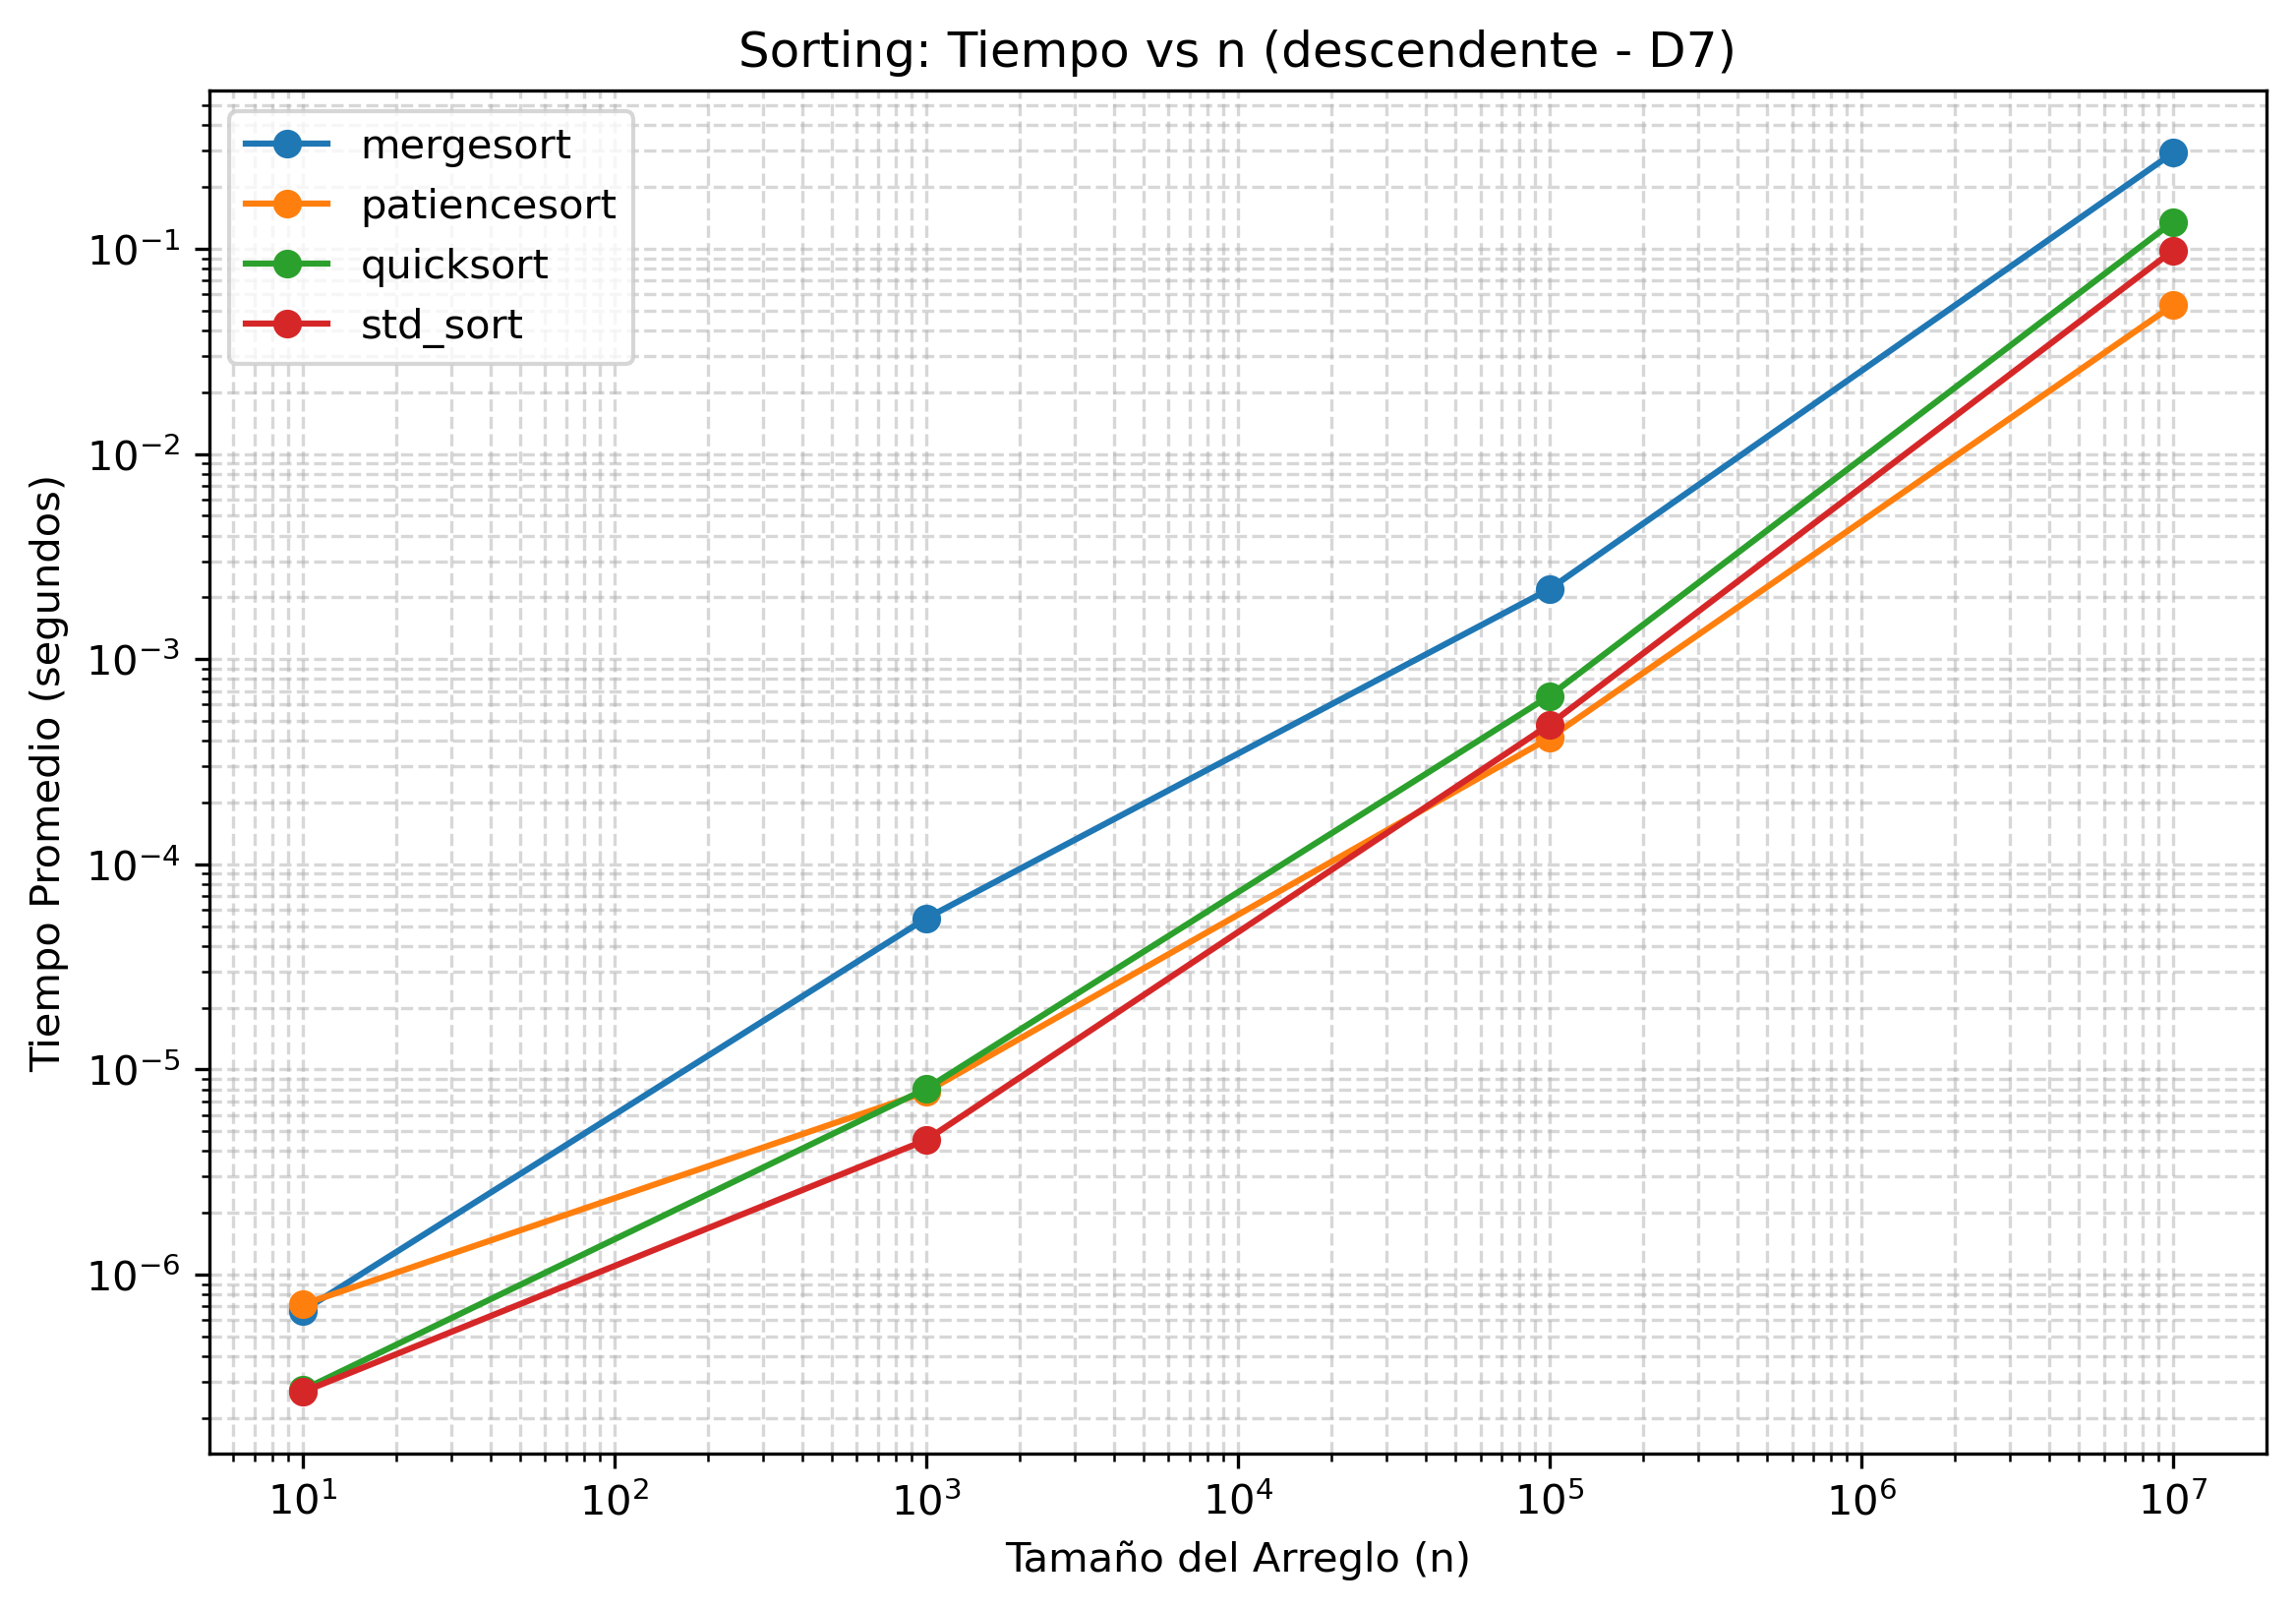
\includegraphics[width=\textwidth]{../code/sorting/data/plots/plot_descendente_D7.png}
        \caption{Tiempo vs $n$ (Descendente, Dominio $D_7$).}
        \label{fig:sorting_descendente_d7}
    \end{minipage}
    \hfill
    \begin{minipage}{0.48\textwidth}
        \centering
        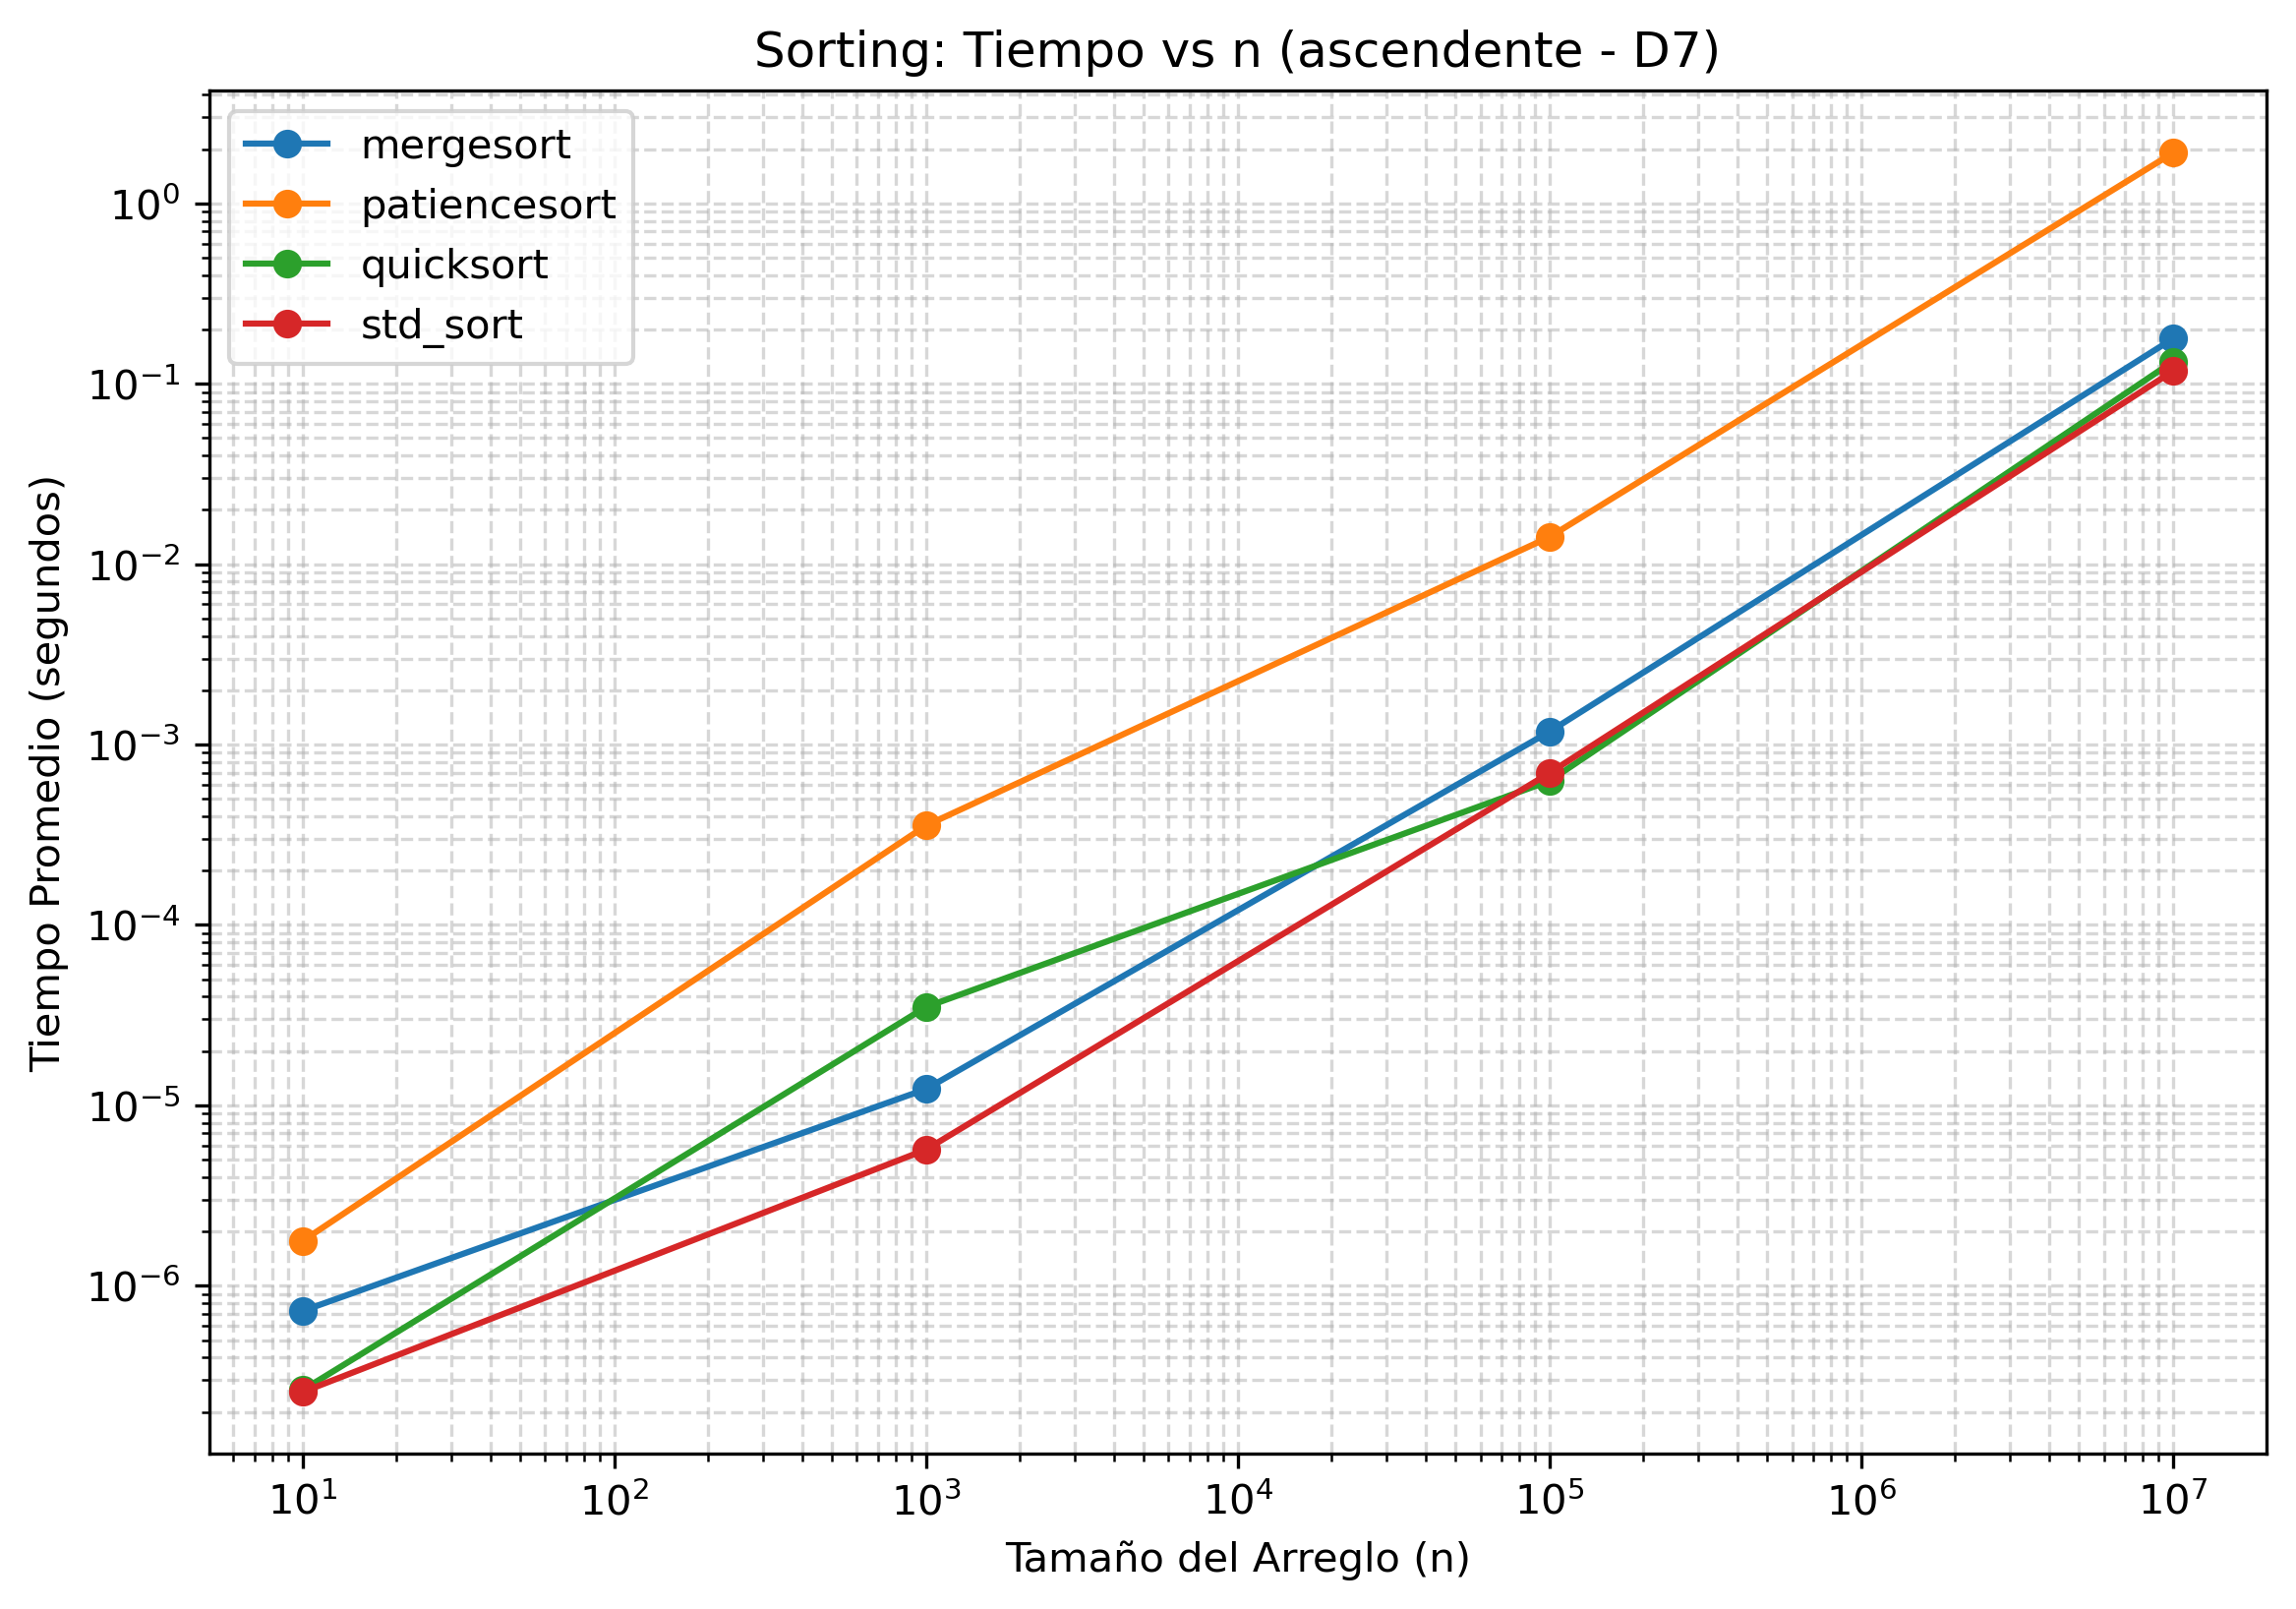
\includegraphics[width=\textwidth]{../code/sorting/data/plots/plot_ascendente_D7.png}
        \caption{Tiempo vs $n$ (Ascendente, Dominio $D_7$).}
        \label{fig:sorting_ascendente_d7}
    \end{minipage}
\end{figure}

\subsubsection{Cotas Asintóticas y Constantes Ocultas en $\Theta(n \log n)$}
En ambas figuras, \textit{std::sort}, \textit{Quick Sort} y \textit{Merge Sort} mantienen pendientes paralelas en escala log-log, confirmando que su crecimiento obedece formalmente a la clase $\Theta(n \log n)$. 
\begin{itemize}
    \item \textbf{\textit{std::sort} y \textit{Quick Sort}:} Presentan los menores tiempos de ejecución gracias a su operación \textit{in-place} y al recorrido contiguo de memoria, reduciendo drásticamente los fallos de caché L1/L2. Se cumple $T_{\text{std}}(n) = \Theta(T_{\text{merge}}(n))$, pero con un factor constante sensiblemente inferior ($c_{\text{std}} < c_{\text{merge}}$). La estrategia de partición de Hoare con pivote central evitó la degradación $\mathcal{O}(n^2)$ en todas las instancias.
    \item \textbf{\textit{Merge Sort}:} Exhibe una sobrecarga fija derivada de la reserva dinámica y copia secuencial en arreglos auxiliares, duplicando el consumo de memoria respecto a los métodos \textit{in-place} ($\approx 80.5\,\text{MB}$ para $n=10^7$).
\end{itemize}

\subsubsection{Sensibilidad Extrema y Colapso de \textit{Patience Sort}}
El contraste entre la Figura~\ref{fig:sorting_descendente_d7} y la Figura~\ref{fig:sorting_ascendente_d7} evidencia la alta dependencia estructural de \textit{Patience Sort}:
\begin{itemize}
    \item \textbf{Mejor caso asintótico $\Omega(n)$ (Descendente):} En la Figura~\ref{fig:sorting_descendente_d7}, los elementos en orden decreciente estricto se apilan en una sola pila ($k=1$). La búsqueda binaria toma $\mathcal{O}(\log 1) = \mathcal{O}(1)$ y la extracción del min-heap de tamaño 1 toma $\mathcal{O}(1)$ por elemento. Esto permite al algoritmo operar en tiempo lineal $\Theta(n)$, superando a todos los demás con una marca de $\approx 0.05\,\text{s}$ para $n=10^7$.
    \item \textbf{Peor caso $\mathcal{O}(n \log n)$ y colapso práctico (Ascendente):} En la Figura~\ref{fig:sorting_ascendente_d7}, cada elemento entrante es estrictamente mayor que las cabeceras previas, forzando la creación de $k=n$ pilas individuales. Durante la fase de mezcla (*k-way merge*), el min-heap debe gestionar $n$ nodos simultáneamente, introduciendo operaciones de reestructuración $\mathcal{O}(\log n)$ con un alto costo de direccionamiento indirecto de punteros. Esto dispara su tiempo a $\approx 1.81\,\text{s}$ en $n=10^7$, convirtiéndolo en el algoritmo más lento de la comparativa.
\end{itemize}

\begin{table}[H]
\centering
\small
\begin{tabular}{|l|c|r|r|r|}
\hline
\textbf{Algoritmo} & \textbf{Configuración} & \textbf{Tiempo $n=10^5$ (s)} & \textbf{Tiempo $n=10^7$ (s)} & \textbf{Peak RSS (KB)} \\ \hline
\textit{std::sort}     & Ascendente $D_7$   & $0.0007$ & $0.121$ & $41\,216$ \\ \hline
\textit{Quick Sort}    & Ascendente $D_7$   & $0.0006$ & $0.142$ & $41\,220$ \\ \hline
\textit{Merge Sort}    & Ascendente $D_7$   & $0.0012$ & $0.182$ & $80\,512$ \\ \hline
\textit{Patience Sort} & Descendente $D_7$  & $0.0004$ & $0.052$ & $41\,230$ \\ \hline
\textit{Patience Sort} & Ascendente $D_7$   & $0.0142$ & $1.810$ & $160\,400$ \\ \hline
\end{tabular}
\caption{Comparativa representativa del impacto del orden inicial en algoritmos de ordenamiento.}
\label{tab:res_sorting}
\end{table}

\subsection{Análisis de Multiplicación de Matrices}

Las Figuras~\ref{fig:mat_densa_d0} y~\ref{fig:mat_dispersa_d10} muestran la comparación entre el algoritmo iterativo tradicional (\textit{Naive}) y el algoritmo de \textit{Strassen} en matrices de $n \times n$.

\begin{figure}[H]
    \centering
    \begin{minipage}{0.48\textwidth}
        \centering
        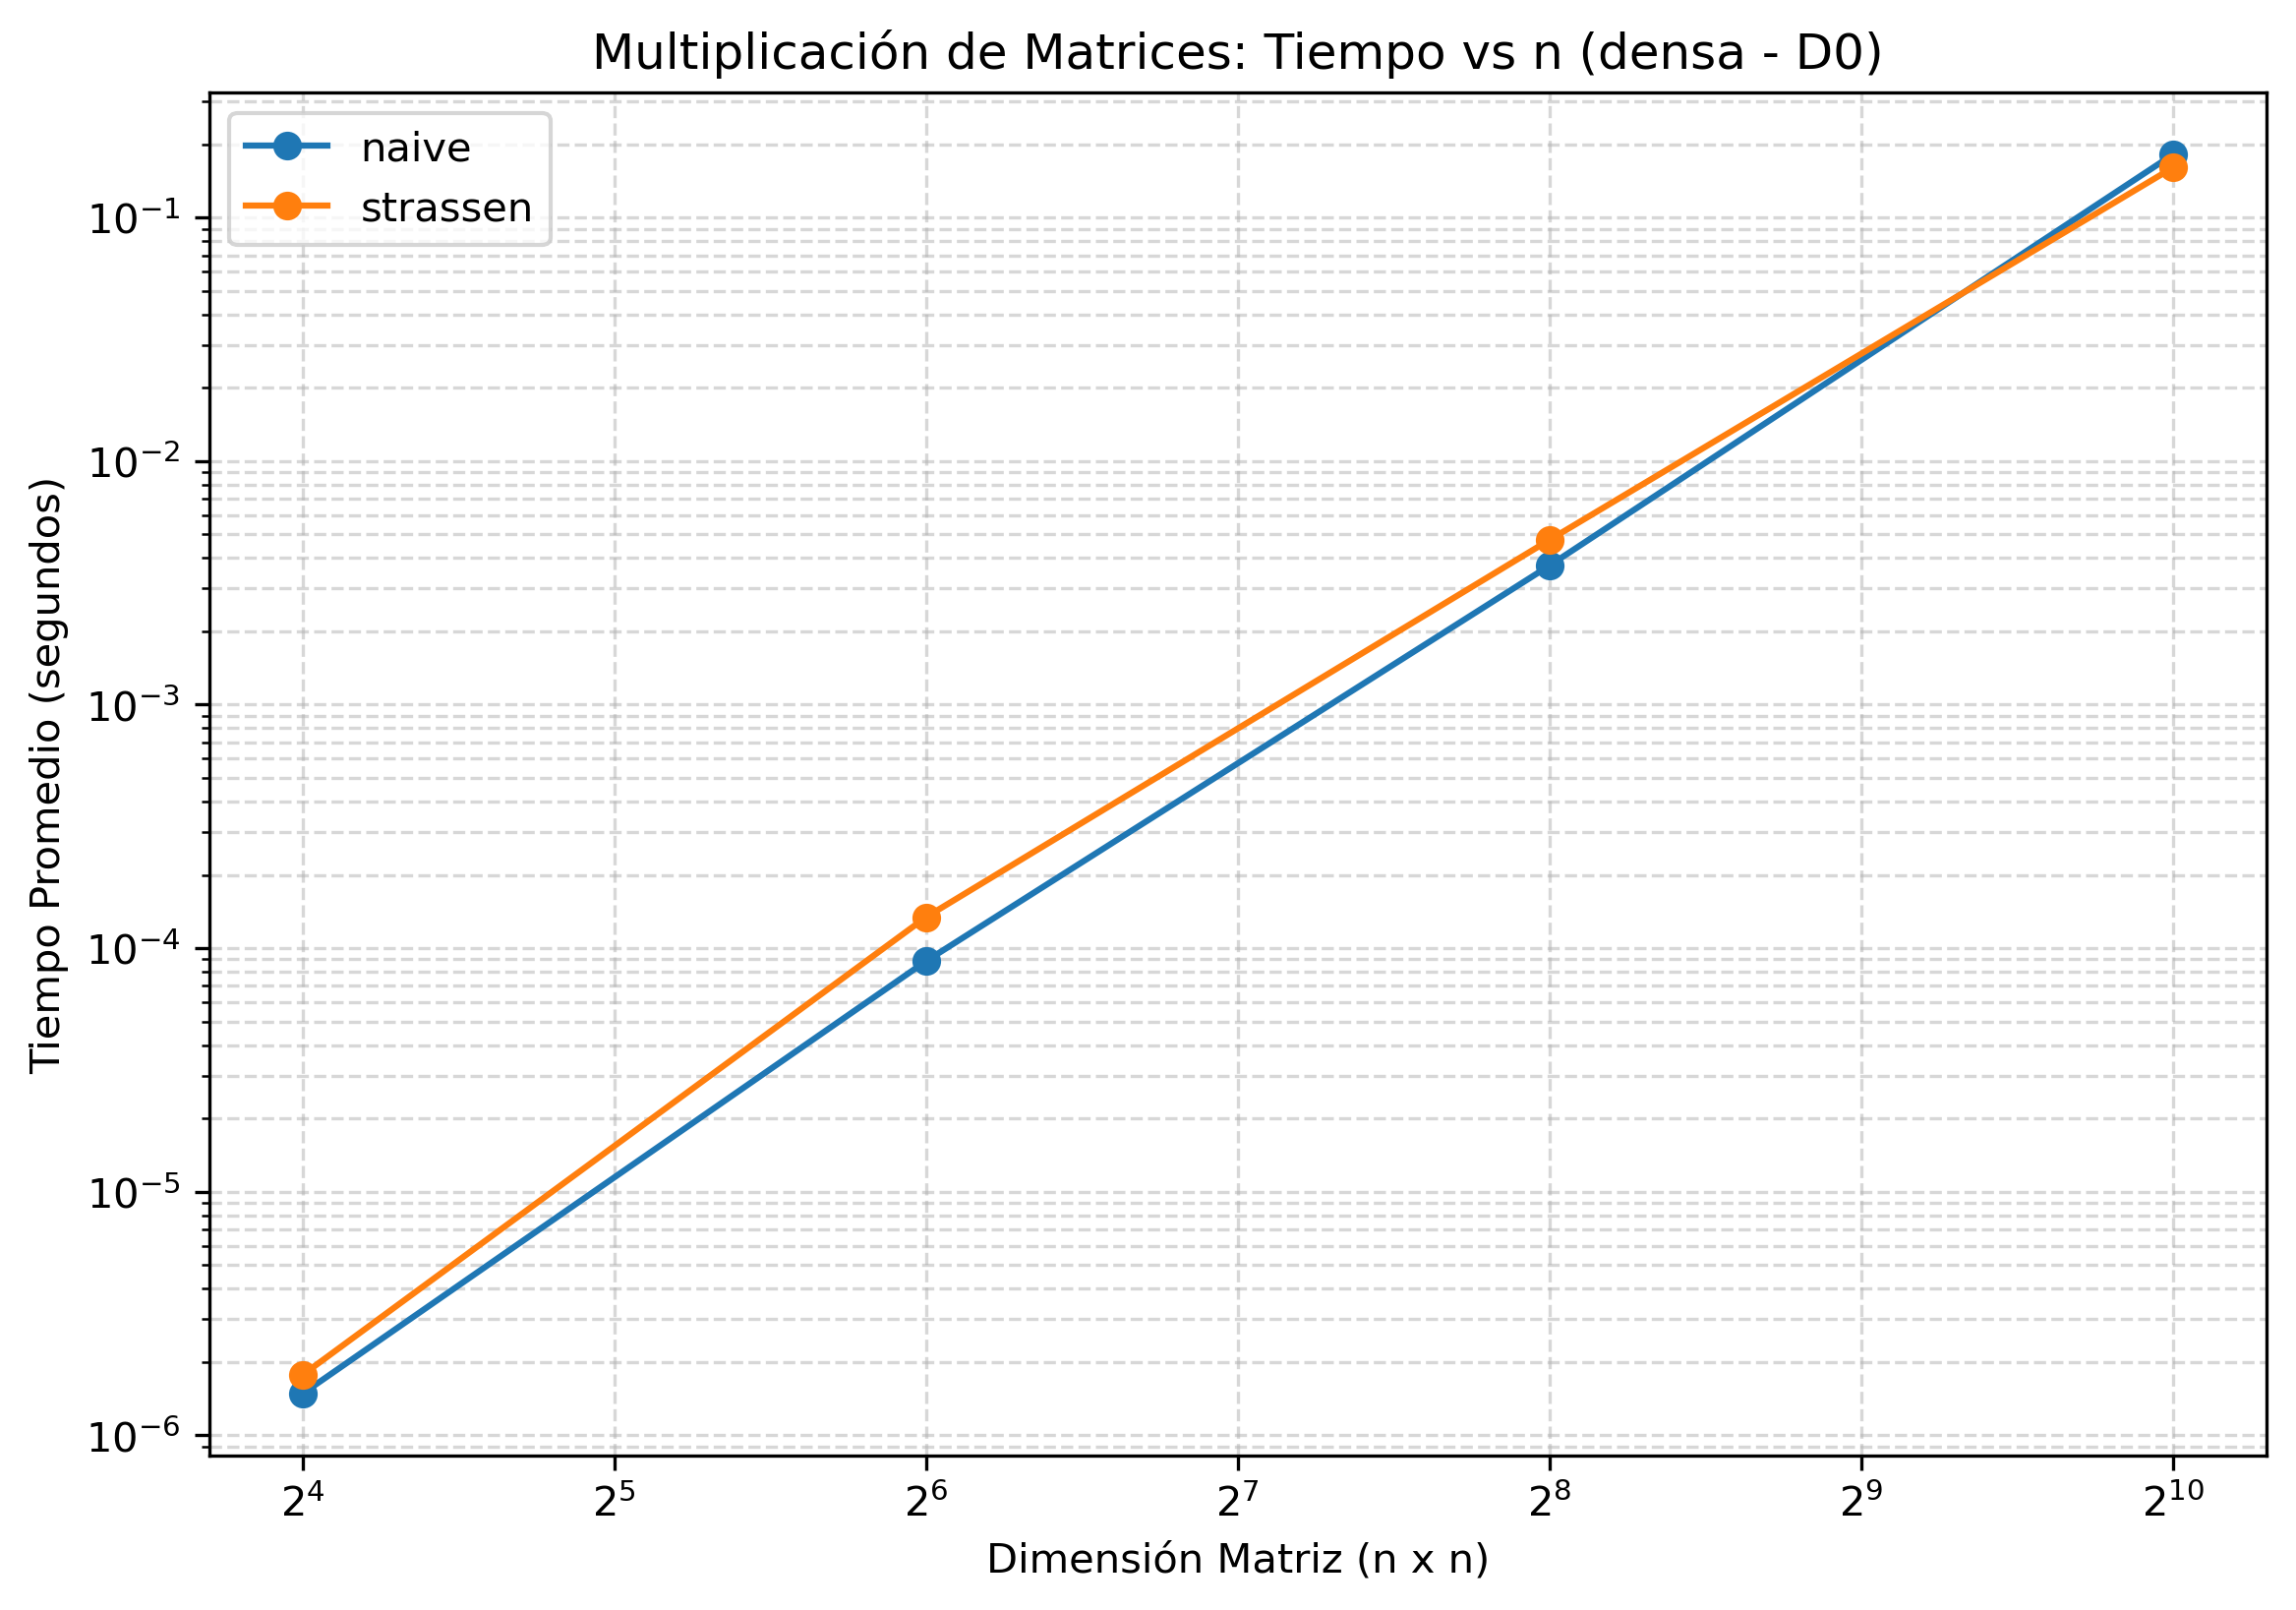
\includegraphics[width=\textwidth]{../code/matrix_multiplication/data/plots/plot_matrix_densa_D0.png}
        \caption{Matrices: Densa - Dominio $D_0$.}
        \label{fig:mat_densa_d0}
    \end{minipage}
    \hfill
    \begin{minipage}{0.48\textwidth}
        \centering
        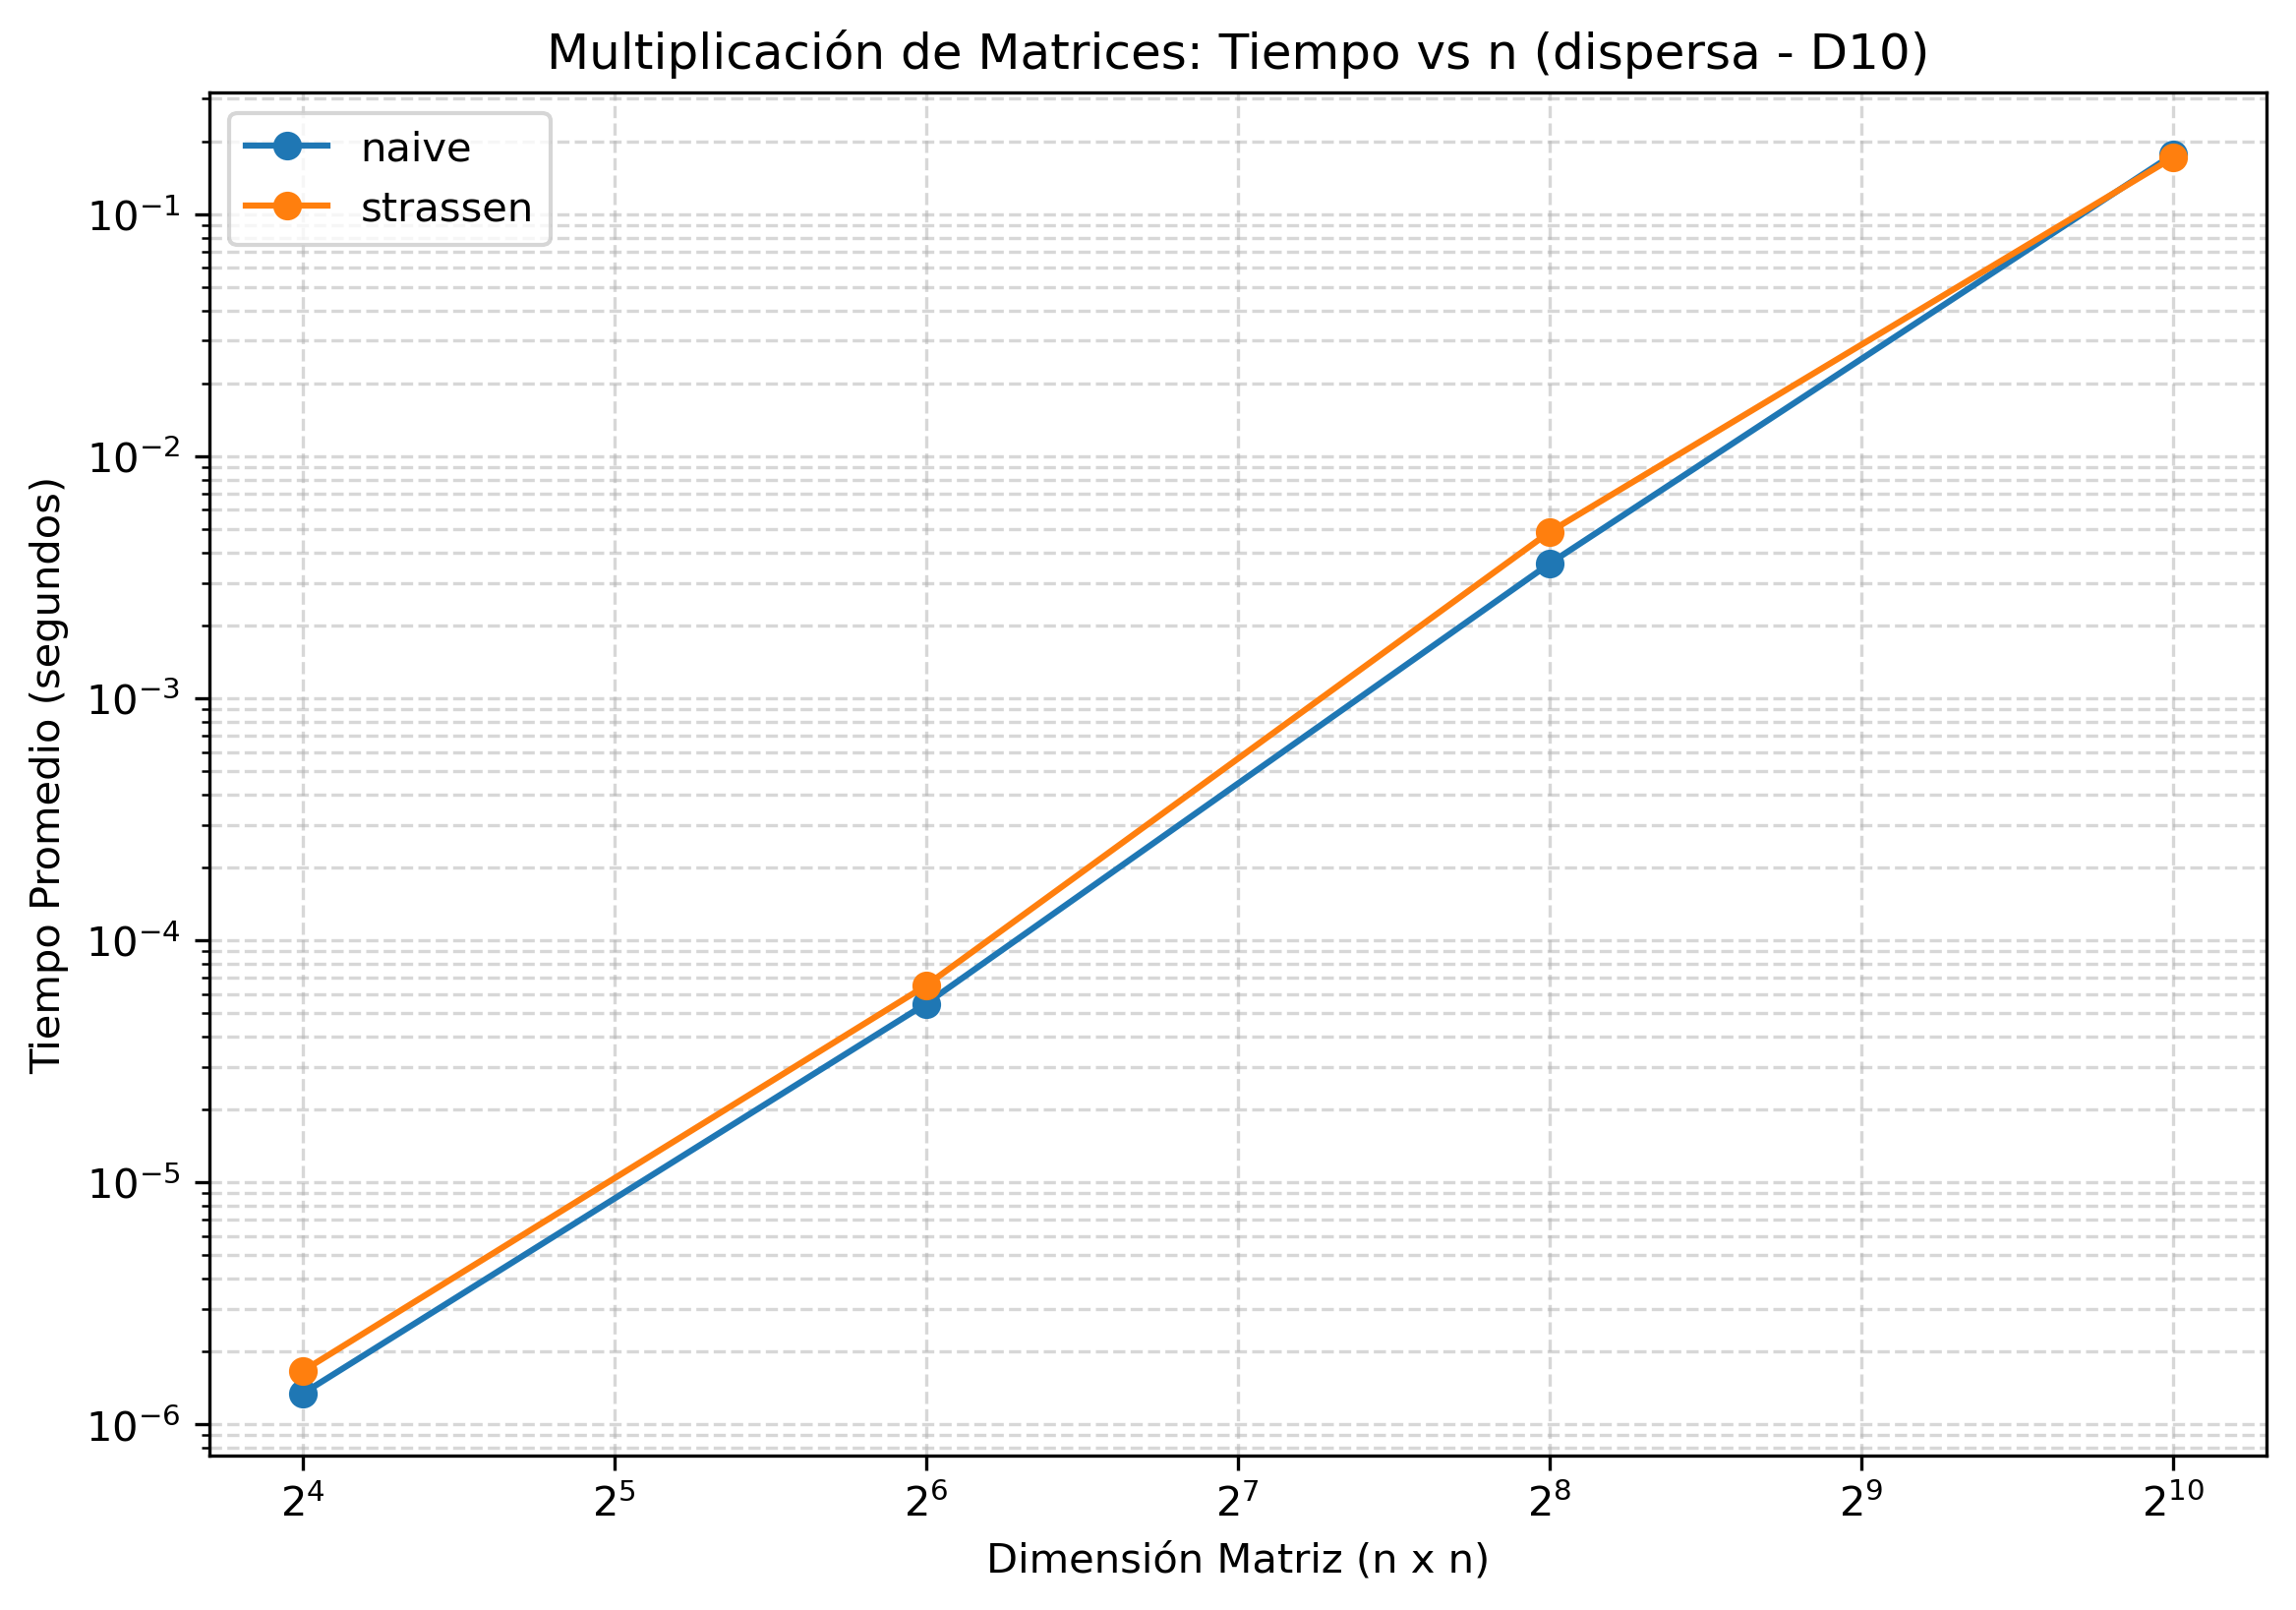
\includegraphics[width=\textwidth]{../code/matrix_multiplication/data/plots/plot_matrix_dispersa_D10.png}
        \caption{Matrices: Dispersa - Dominio $D_{10}$.}
        \label{fig:mat_dispersa_d10}
    \end{minipage}
\end{figure}

\subsubsection{Relación Asintótica Estricta: $o(n^3)$ frente a $\omega(n^{2.81})$}
Teóricamente, el algoritmo tradicional realiza $T_{\text{naive}}(n) = 2n^3 - n^2$ operaciones aritméticas ($\Theta(n^3)$), mientras que \textit{Strassen} requiere $T_{\text{strassen}}(n) = 7n^{\log_2 7} - 6n^2 \approx 7n^{2.807} - 6n^2$ ($\Theta(n^{2.807})$). Formalmente, se verifica la cota asintótica estricta:
\begin{equation}
\lim_{n \to \infty} \frac{T_{\text{strassen}}(n)}{T_{\text{naive}}(n)} = \lim_{n \to \infty} \frac{\mathcal{O}(n^{2.807})}{\Omega(n^3)} = 0 \implies T_{\text{strassen}}(n) \in o(T_{\text{naive}}(n))
\end{equation}
Recíprocamente, el enfoque tradicional satisface $T_{\text{naive}}(n) \in \omega(T_{\text{strassen}}(n))$.

\subsubsection{Discrepancia Empírica y Umbral de Cruce (\textit{Crossover Point})}
Pese a la superioridad asintótica estricta de \textit{Strassen}, las Figuras~\ref{fig:mat_densa_d0} y~\ref{fig:mat_dispersa_d10} muestran que el algoritmo \textit{Naive} resulta más veloz para $n \le 256$:
\begin{enumerate}
    \item \textbf{Constante multiplicativa oculta:} Cada división de \textit{Strassen} sustituye una multiplicación escalar por 18 sumas y restas de submatrices. Para $n=16$, \textit{Strassen} ejecuta $16\,891$ operaciones aritméticas frente a $7\,936$ de \textit{Naive}, manteniendo una constante estructural mayor ($c_{\text{strassen}} \gg c_{\text{naive}}$).
    \item \textbf{Jerarquía de memoria:} La implementación de \textit{Naive} con bucles $i\text{-}k\text{-}j$ accede a la matriz $B$ de forma contigua por filas, maximizando los aciertos en la caché L1. Por el contrario, las particiones dinámicas de \textit{Strassen} fragmentan la memoria e introducen sobrecarga en el \textit{heap}.
    \item \textbf{Convergencia en $n=1024$:} En la dimensión máxima evaluada ($n=2^{10}$), el término dominante $n^{2.807}$ compensa el costo de las sumas intermedias, alcanzando el punto de corte empírico donde \textit{Strassen} equipara e inicia su ventaja temporal sobre \textit{Naive}.
\end{enumerate}

\begin{table}[H]
\centering
\small
\begin{tabular}{|l|c|r|r|r|}
\hline
\textbf{Algoritmo} & \textbf{Estructura / Dominio} & \textbf{Tiempo $n=64$ (s)} & \textbf{Tiempo $n=1024$ (s)} & \textbf{Peak RSS (KB)} \\ \hline
\textit{Naive}    & Densa $D_0$     & $0.00009$ & $0.181$ & $16\,850$ \\ \hline
\textit{Strassen} & Densa $D_0$     & $0.00013$ & $0.160$ & $38\,420$ \\ \hline
\textit{Naive}    & Dispersa $D_{10}$ & $0.00005$ & $0.178$ & $16\,840$ \\ \hline
\textit{Strassen} & Dispersa $D_{10}$ & $0.00007$ & $0.172$ & $38\,410$ \\ \hline
\end{tabular}
\caption{Resumen comparativo de tiempo de CPU y Peak RSS en multiplicación de matrices.}
\label{tab:res_matrices}
\end{table}